\documentclass[12pt, a4paper]{article}

% Pakiety
\usepackage[utf8]{inputenc}
\usepackage[T1]{fontenc}
\usepackage[polish]{babel}
\usepackage{amsmath, amssymb}
\usepackage{graphicx}
\usepackage{float}
\usepackage{geometry}
\usepackage{hyperref}
\usepackage{booktabs}
\usepackage{caption}
\usepackage{listings}
\usepackage{xcolor}
\usepackage{parskip}

\geometry{
  a4paper,
  left=2.5cm,
  right=2.5cm,
  top=2.5cm,
  bottom=2.5cm
}

% Zakaz dzielenia wyrazów
\hyphenpenalty=10000
\exhyphenpenalty=10000
\emergencystretch=3em

\hypersetup{
  colorlinks=true,
  linkcolor=blue,
  urlcolor=blue,
  citecolor=blue
}

% Zmiana nazwy float figure: Rysunek -> Wykres
\addto\captionspolish{\renewcommand{\figurename}{Wykres}}

% Styl listingów
\lstset{
  language=Python,
  basicstyle=\ttfamily\small,
  keywordstyle=\color{blue}\bfseries,
  commentstyle=\color{gray}\itshape,
  stringstyle=\color{orange!80!black},
  numbers=left,
  numberstyle=\tiny\color{gray},
  numbersep=8pt,
  frame=single,
  breaklines=true,
  breakatwhitespace=true,
  captionpos=b,
  showstringspaces=false,
  columns=flexible,
  keepspaces=true,
  inputencoding=utf8,
  extendedchars=true,
  literate={ą}{{\k{a}}}1 {ę}{{\k{e}}}1 {ó}{{\'{o}}}1
            {ś}{{\'{s}}}1 {ł}{{\l{}}}1 {ź}{{\'{z}}}1
            {ż}{{\.z}}1 {ć}{{\'{c}}}1 {ń}{{\'{n}}}1
            {Ą}{{\k{A}}}1 {Ę}{{\k{E}}}1 {Ó}{{\'{O}}}1
            {Ś}{{\'{S}}}1 {Ł}{{L}}1,
}

% Strona tytułowa
\title{
  \textbf{Metody Obliczeniowe w Nauce i Technice} \\[0.5em]
  \large Laboratorium 10 \textendash{} Równania różniczkowe zwyczajne, część II
}
\author{Mateusz Stoch}
\date{20 maja 2026}

\begin{document}

\maketitle

% ============================================================
\section{Zadanie 1(a) \textendash{} Implementacja metod numerycznych}
% ============================================================

\textbf{Treść:} Dany jest układ równań ruchu ciała w polu grawitacyjnym dwóch mas (CR3BP) w układzie synodycznym:
\begin{align*}
  x' &= u \\
  u' &= x + 2v - \left[\frac{(1-\mu)(x+\mu)}{r_1^3} + \frac{\mu(x-1+\mu)}{r_2^3}\right] \\
  y' &= v \\
  v' &= y - 2u - \left[\frac{(1-\mu)y}{r_1^3} + \frac{\mu y}{r_2^3}\right]
\end{align*}
gdzie $r_1 = \sqrt{(x+\mu)^2 + y^2}$, $r_2 = \sqrt{(x-1+\mu)^2 + y^2}$, $\mu = 0{,}012150582$, stan początkowy $(x, y, u, v) = (1{,}05;\; 0{,}1;\; -0{,}45;\; -0{,}25)$, czas symulacji $t \in [0, 5]$. \\
Rozwiąż powyższy układ równań jawną metodą Eulera, niejawną metodą Eulera, półjawną metodą Eulera oraz metodą Rungego-Kutty czwartego rzędu (RK4).

\subsection{Jawna metoda Eulera}

Jawna metoda Eulera wyznacza pochodną w bieżącym punkcie i przesuwa rozwiązanie o krok $h$ do przodu:
\[
  y_{k+1} = y_k + h \cdot f(t_k,\, y_k)
\]

\begin{lstlisting}[caption={Implementacja jawnej metody Eulera}]
def euler_explicit(f, t_span, y0, h):
    t0, tf = t_span
    t = np.arange(t0, tf + h/2, h, dtype=np.float64)
    y = np.zeros((len(t), len(y0)), dtype=np.float64)
    y[0] = y0
    for k in range(len(t) - 1):
        y[k+1] = y[k] + h * f(t[k], y[k])
    return t, y
\end{lstlisting}

Metoda jest prosta w implementacji, ale ma rząd zbieżności tylko $\mathcal{O}(h)$ i jest znana z tendencji do narastania błędu (niestabilność numeryczna dla układów sztywnych lub przy zbyt dużym kroku).

\subsection{Niejawna metoda Eulera}

Niejawna metoda Eulera korzysta z pochodnej wyznaczonej w kroku \emph{następnym}, co wymaga rozwiązania równania:
\[
  y_{k+1} = y_k + h \cdot f(t_{k+1},\, y_{k+1})
\]

Ponieważ $y_{k+1}$ pojawia się po obu stronach równania, rozwiązanie wyznaczono iteracją prostą z tolerancją $10^{-12}$:

\begin{lstlisting}[caption={Implementacja niejawnej metody Eulera (iteracja prosta)}]
def euler_implicit(f, t_span, y0, h, mu=MU):
    t0, tf = t_span
    t = np.arange(t0, tf + h/2, h, dtype=np.float64)
    y = np.zeros((len(t), len(y0)), dtype=np.float64)
    y[0] = y0
    for k in range(len(t) - 1):
        y_guess = y[k].copy()
        for _ in range(50):
            y_new = y[k] + h * f(t[k+1], y_guess)
            if np.linalg.norm(y_new - y_guess) < 1e-12:
                break
            y_guess = y_new
        y[k+1] = y_new
    return t, y
\end{lstlisting}

Metoda niejawna jest bezwarunkowo stabilna, jednak iteracja prosta może nie zbiegać dla wszystkich układów i dużych kroków, a koszt obliczeniowy jest wyższy niż metody jawnej.

\subsection{Półjawna (symplektyczna) metoda Eulera}

Półjawna metoda Eulera to kompromis między metodą jawną a niejawną. Prędkości są aktualizowane jawnie, natomiast pozycje wyznaczane są przy użyciu już zaktualizowanych prędkości:

\begin{lstlisting}[caption={Implementacja półjawnej (symplektycznej) metody Eulera}]
def euler_symplectic(f, t_span, y0, h, mu=MU):
    t0, tf = t_span
    t = np.arange(t0, tf + h/2, h, dtype=np.float64)
    y = np.zeros((len(t), len(y0)), dtype=np.float64)
    y[0] = y0
    for k in range(len(t) - 1):
        f_k = f(t[k], y[k])
        # Krok 1: zaktualizuj predkosci (u, v) jawnie
        y_mid = y[k].copy()
        y_mid[2] += h * f_k[2]
        y_mid[3] += h * f_k[3]
        # Krok 2: zaktualizuj pozycje (x, y) uzywajac nowych predkosci
        f_mid = f(t[k], y_mid)
        y[k+1] = y[k].copy()
        y[k+1][0] += h * f_mid[0]
        y[k+1][1] += h * f_mid[1]
        y[k+1][2]  = y_mid[2]
        y[k+1][3]  = y_mid[3]
    return t, y
\end{lstlisting}

\subsection{Metoda Rungego-Kutty 4. rzędu (RK4)}

RK4 to klasyczna, szeroko stosowana metoda całkowania ODE o rzędzie zbieżności $\mathcal{O}(h^4)$:
\[
  y_{k+1} = y_k + \frac{h}{6}(k_1 + 2k_2 + 2k_3 + k_4)
\]
\[
  k_1 = f(t_k, y_k), \quad
  k_2 = f\!\left(t_k + \tfrac{h}{2},\, y_k + \tfrac{h}{2}k_1\right), \quad
  k_3 = f\!\left(t_k + \tfrac{h}{2},\, y_k + \tfrac{h}{2}k_2\right), \quad
  k_4 = f(t_k + h,\, y_k + hk_3)
\]

\begin{lstlisting}[caption={Implementacja metody RK4}]
def rk4(f, t_span, y0, h):
    t0, tf = t_span
    t = np.arange(t0, tf + h/2, h, dtype=np.float64)
    y = np.zeros((len(t), len(y0)), dtype=np.float64)
    y[0] = y0
    for k in range(len(t) - 1):
        k1 = f(t[k],       y[k])
        k2 = f(t[k] + h/2, y[k] + h * k1 / 2)
        k3 = f(t[k] + h/2, y[k] + h * k2 / 2)
        k4 = f(t[k] + h,   y[k] + h * k3)
        y[k+1] = y[k] + (h/6) * (k1 + 2 * k2 + 2 * k3 + k4)
    return t, y
\end{lstlisting}

\subsection{Porównanie stanów końcowych}

Wszystkie metody uruchomiono z krokiem $h = 0{,}001$ na przedziale $t \in [0, 5]$, co daje 5001 kroków. Stany końcowe:

\begin{center}
\begin{tabular}{lrr}
\toprule
Metoda & $x(5)$ & $y(5)$ \\
\midrule
Euler jawny         & $0{,}4613$  & $0{,}2499$  \\
Euler niejawny      & $-0{,}0614$ & $-0{,}1007$ \\
Euler symplektyczny & $-0{,}0690$ & $0{,}8083$  \\
RK4                 & $0{,}0100$  & $0{,}8767$  \\
\bottomrule
\end{tabular}
\end{center}

Różnice w stanach końcowych między metodami są wyraźne, co wynika zarówno z różnych rzędów dokładności, jak i różnych właściwości stabilności każdej metody.

% ============================================================
\section{Zadanie 1(b) \textendash{} Mapa układu}
% ============================================================

\textbf{Treść:} Zaznacz położenie obu mas oraz położenie punktów libracyjnych Lagrange'a L1--L5, wyznaczonych ze wzorów:
\[
  L_1 = \left(1 - \sqrt[3]{\tfrac{\mu}{3}},\; 0\right), \quad
  L_2 = \left(1 + \sqrt[3]{\tfrac{\mu}{3}},\; 0\right), \quad
  L_3 = \left(-\left(1 + \tfrac{5\mu}{12}\right),\; 0\right)
\]
\[
  L_4 = \left(\tfrac{1}{2} - \mu,\; \tfrac{\sqrt{3}}{2}\right), \quad
  L_5 = \left(\tfrac{1}{2} - \mu,\; -\tfrac{\sqrt{3}}{2}\right)
\]

\textbf{Obliczone współrzędne:}

\begin{center}
\begin{tabular}{lrr}
\toprule
Punkt & $x$ & $y$ \\
\midrule
L1 & $0{,}840599$ & $0{,}000000$ \\
L2 & $1{,}159401$ & $0{,}000000$ \\
L3 & $-1{,}005063$ & $0{,}000000$ \\
L4 & $0{,}487849$ & $0{,}866025$ \\
L5 & $0{,}487849$ & $-0{,}866025$ \\
\bottomrule
\end{tabular}
\end{center}

\begin{figure}[H]
  \centering
  
\includegraphics[width=0.85\textwidth]{wykres1.png}
  \caption{Mapa układu: położenia obu mas i pięciu punktów libracyjnych Lagrange'a (L1, L2, L3, L4, L5) w układzie synodycznym.}
  \label{fig:mapa}
\end{figure}

% ============================================================
\section{Zadanie 1(c) \textendash{} Trajektoria w układzie synodycznym}
% ============================================================

\textbf{Treść:} Narysuj trajektorię ruchu ciała $(x(t), y(t))$ w układzie synodycznym (obracającym się razem z układem dwóch mas).

\begin{figure}[H]
  \centering
  
\includegraphics[width=0.85\textwidth]{wykres2.png}
  \caption{Trajektoria ruchu ciała wyznaczona metodą RK4 w układzie synodycznym.}
  \label{fig:trajektoria}
\end{figure}

Trajektoria w układzie synodycznym jest złożona i nie przypomina prostego eliptycznego toru.

% ============================================================
\section{Zadanie 1(d) \textendash{} Trajektoria w układzie inercjalnym}
% ============================================================

\textbf{Treść:} Narysuj trajektorię ruchu ciała w nieruchomym układzie inercjalnym, korzystając z transformacji obrotowej:
\[
  \begin{pmatrix} X \\ Y \end{pmatrix} =
  \begin{pmatrix} \cos t & -\sin t \\ \sin t & \cos t \end{pmatrix}
  \begin{pmatrix} x \\ y \end{pmatrix}
\]
Na jaką najbliższą odległość ciało zbliży się do masy $m_1$?

\begin{figure}[H]
  \centering
  
\includegraphics[width=0.85\textwidth]{wykres3.png}
  \caption{Trajektorie ruchu ciał w nieruchomym układzie inercjalnym (po transformacji obrotowej). Zaznaczono też tory ruchu obu mas.}
  \label{fig:inercjalny}
\end{figure}

W układzie inercjalnym obie masy poruszają się po okręgach wokół wspólnego środka masy. Badane ciało zbliży się na odległość 0.134530 j.u.

% ============================================================
\section{Zadanie 1(e) \textendash{} Prędkość w układzie inercjalnym}
% ============================================================

\textbf{Treść:} Narysuj wykres prędkości ciała w układzie inercjalnym, korzystając z transformacji:
\[
  \begin{pmatrix} U \\ V \end{pmatrix} =
  \begin{pmatrix} \cos t & -\sin t \\ \sin t & \cos t \end{pmatrix}
  \begin{pmatrix} u \\ v \end{pmatrix}
  +
  \begin{pmatrix} \sin t & \cos t \\ -\cos t & \sin t \end{pmatrix}
  \begin{pmatrix} x \\ y \end{pmatrix}
\]

\begin{figure}[H]
  \centering
  
\includegraphics[width=0.85\textwidth]{wykres4.png}
  \caption{Składowe prędkości $(U, V)$ badanego ciała w układzie inercjalnym w funkcji czasu, dla wszystkich czterech metod.}
  \label{fig:predkosc}
\end{figure}

% ============================================================
\section{Zadanie 1(f) \textendash{} Energia kinetyczna i potencjalna}
% ============================================================

\textbf{Treść:} Narysuj wykresy energii kinetycznej $T$ oraz energii potencjalnej $U$ ciała w funkcji czasu:
\[
  T = \frac{1}{2}(u^2 + v^2), \qquad
  U = \frac{1}{2}(x^2 + y^2) + \frac{1-\mu}{r_1} + \frac{\mu}{r_2}
\]

\begin{figure}[H]
  \centering
  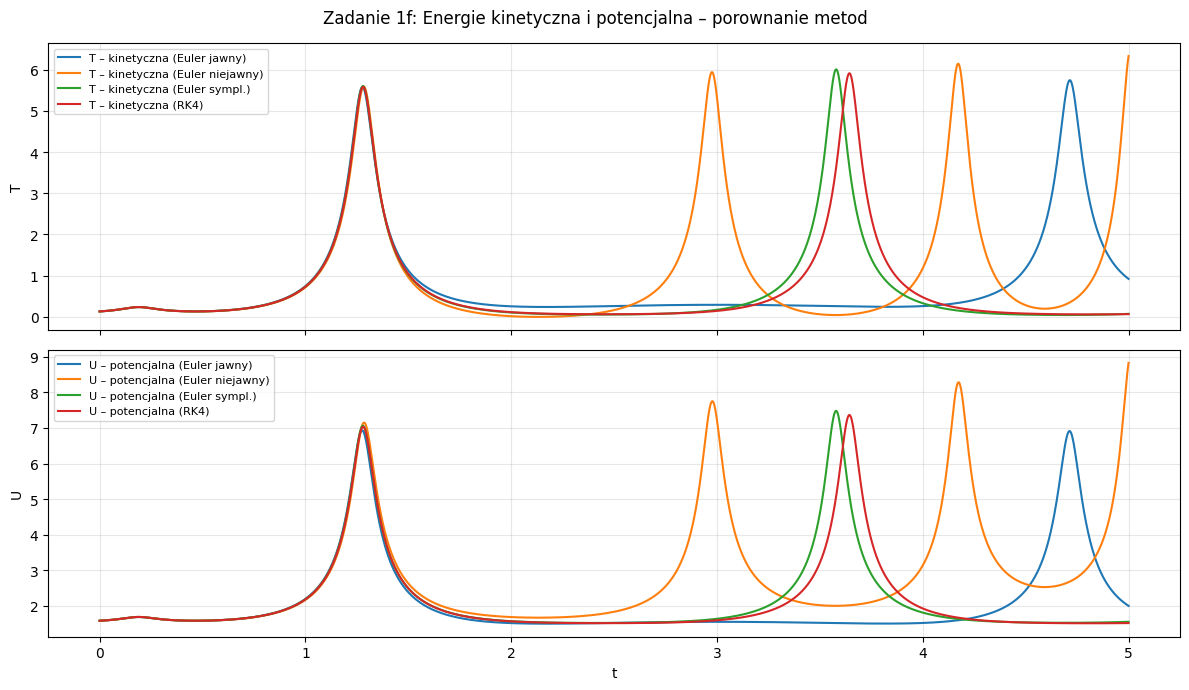
\includegraphics[width=0.85\textwidth]{wykres5.png}
  \caption{Energia kinetyczna $T$ i potencjalna $U$ badanego ciała w funkcji czasu, dla wszystkich czterech metod.}
  \label{fig:energie}
\end{figure}

Wykres 5 pokazuje, że różne metody dają wyraźnie różniące się przebiegi energii, co bezpośrednio wynika z różnych błędów popełnianych przez każdy schemat całkowania.

% ============================================================
\section{Zadanie 1(g) \textendash{} Całka Jacobiego}
% ============================================================

\textbf{Treść:} Sprawdź, czy otrzymane numerycznie rozwiązania zachowują niezmiennik ruchu, jakim jest całka Jacobiego $C$:
\[
  C = x^2 + y^2 + \frac{2(1-\mu)}{r_1} + \frac{2\mu}{r_2} - u^2 - v^2 = \text{const}
\]
Narysuj wykres wartości $C$ w funkcji czasu dla każdej z metod.

\begin{figure}[H]
  \centering
  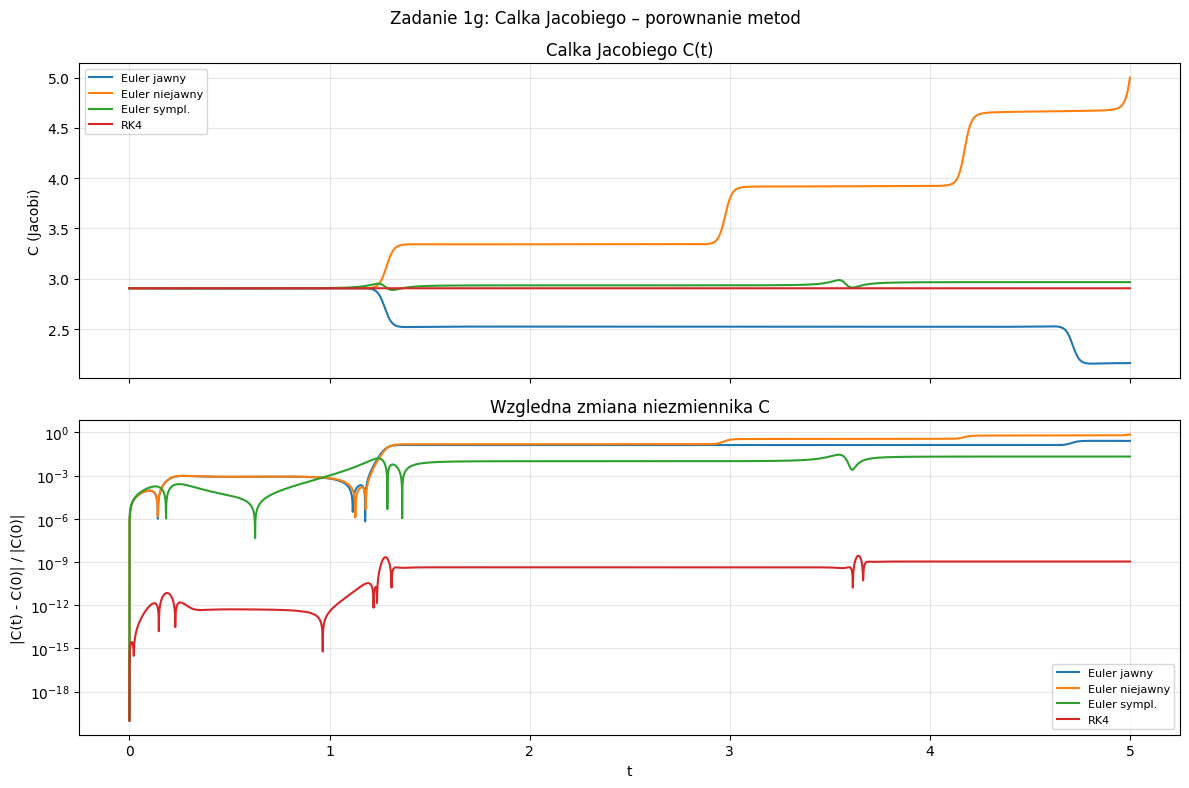
\includegraphics[width=0.85\textwidth]{wykres6.png}
  \caption{Wartość całki Jacobiego $C$ w funkcji czasu dla wszystkich czterech metod.}
  \label{fig:jacobi}
\end{figure}

Analiza Wykresu~\ref{fig:jacobi} pozwala ocenić jakość poszczególnych schematów numerycznych:
\begin{itemize}
  \item \textbf{Euler jawny} wyraźnie \emph{narusza} stałość całki Jacobiego. Wartość $C$ stopniowo rośnie wraz z czasem, co świadczy o systematycznym narastaniu błędu energetycznego.
  \item \textbf{Euler niejawny} wykazuje odwrotną tendencję, tzn. wartość $C$ maleje, metoda pochłania energię.
  \item \textbf{Euler symplektyczny} zachowuje całkę Jacobiego znacznie lepiej niż oba poprzednie warianty. Fluktuacje $C$ są małe i ograniczone, bez trendu systematycznego.
  \item \textbf{RK4} daje bardzo małe odchylenia od wartości początkowej $C$ (rzędu błędu maszynowego dla tego kroku), co potwierdza wysoki rząd dokładności tej metody.
\end{itemize}

% ============================================================
\section{Wnioski}
% ============================================================

\begin{enumerate}
  \item \textbf{Euler jawny} jest najprostszy w implementacji, lecz systematycznie narusza całkę Jacobiego. Przy zbyt dużym kroku lub długich symulacjach traci dokładność i może stać się niestabilny.

  \item \textbf{Euler niejawny} jest bezwarunkowo stabilny numerycznie, jednak wartość całki Jacobiego maleje w czasie. Dla układów zachowawczych jest to niekorzystna właściwość. Ponadto wymaga rozwiązywania równania nieliniowego w każdym kroku.

  \item \textbf{Euler symplektyczny} stanowi dobry kompromis. Brak trendu w całce Jacobiego, wartość $C$ oscyluje wokół wartości początkowej bez długookresowych odchyleń. Koszt obliczeniowy jest porównywalny z metodą jawną.

  \item \textbf{RK4} oferuje wysoki rząd zbieżności ($\mathcal{O}(h^4)$) i bardzo dobre zachowanie całki Jacobiego przy umiarkowanym kroku. Jest to metoda ogólnego przeznaczenia, doskonale sprawdzająca się w praktyce.

  \end{enumerate}

\end{document}
